\documentclass[doc,floatsintext,donotrepeattitle,letterpaper,12pt]{apa7}

\usepackage[T1]{fontenc}
\usepackage[utf8]{inputenc}
\raggedbottom

\usepackage{csquotes}
\MakeOuterQuote{"}

\usepackage{booktabs}
\usepackage{caption}
\usepackage{setspace}
\captionsetup[figure]{skip=10pt,justification=justified}
\captionsetup[table]{skip=10pt}

\usepackage{hyperref}
\hypersetup{hidelinks,colorlinks=false}
\urlstyle{same}

\usepackage{amsmath}
\usepackage{amsfonts}
\usepackage{amssymb}

\usepackage{tcolorbox}
\usepackage{graphicx}

\usepackage[
  autocite=inline,
  style=apa,
  sortcites=true,
  sorting=nyt,
  backend=biber
  ]{biblatex}
\addbibresource{../references.bib}
\addbibresource{../r-references.bib}

\renewcommand{\postnotedelim}{\space}

\title{Autonomy-supportive instructional language does not enhance skill acquisition compared to controlling instructional language}
\shorttitle{Instructional language and motor skill learning}

\renewcommand\author[1]{}
\renewcommand\affiliation[1]{}
\authorsnames[1, 1, 2, 2, 3, 4, 5, {1,*}]{Laura St. Germain, Brad McKay, Lidia Barbera, Chitrini Tandon, Jewsende Seedu, Chantal Carrillo, Denver M.Y. Brown, Michael J. Carter\vspace{2ex}}
\authorsaffiliations{{Department of Kinesiology, McMaster University}, {School of Interdisciplinary Science, McMaster University}, {Faculty of Health Sciences, McMaster University}, {Department of Psychology, Neuroscience, and Behaviour, McMaster University}, {Department of Psychology, The University of Texas at San Antonio}}


\abstract{Instructional language is one of three techniques in OPTIMAL theory that can be manipulated to foster an autonomy-supportive practice environment to enhance motor performance and learning. While autonomy-supportive language has been shown to be beneficial in educational psychology, coaching, and health settings, the wording of task instructions has received minimal attention in the motor learning literature to date. We investigated the influence of two instructional language styles on skill acquisition in a preregistered experiment. Participants (\emph{N} = 156) learned a speed cup stacking task and received instructions throughout practice that used either autonomy-supportive or controlling language. Although the autonomy-supportive instructions resulted in higher perceptions of autonomy, there were no group differences for motor performance in acquisition or retention. Perceptions of competence and intrinsic motivation did not differ between groups at any time point. These data are difficult to reconcile with key predictions in OPTIMAL theory regarding a direct and causal influence of motivational factors on performance and learning. However, our equivalence test suggests these effects on skill acquisition may be smaller than what we were powered to detect. These findings are consistent with a growing body of evidence highlighting the need for much larger \emph{N} experiments in motor learning research.}

\keywords{Motor learning, Retention, OPTIMAL theory, Preregistered \newline
\hspace*{\fill} \textcolor{orange}{\textbf{\emph{PREPRINT - NOT PEER-REVIEWED}}} \hspace*{\fill}
}

\authornote{\vspace{-1em} \newline
\addORCIDlink{Laura St. Germain}{0000-0002-5513-4183} \newline
\addORCIDlink{Brad McKay}{0000-0002-7408-2323} \newline
\addORCIDlink{Devnver M.Y. Brown}{0000-0003-4078-8253} \newline
\addORCIDlink{Michael J. Carter}{0000-0002-0675-4271} \newline

\noindent *Corresponding author: Michael J. Carter (cartem11@mcmaster.ca; motorlab@mcmaster.ca)
\newline
\begin{tcolorbox}[width=\textwidth,colback={white},colframe=orange,coltext=black]
    \noindent \textbf{Please cite as:} \newline
    St. Germain, L., McKay, B., Barbera, L., Tandon, C., Seedu, J., Carrillo, C., Brown, D.M.Y., \& Carter, M.J. Autonomy-supportive instructional language does not enhance skill acquisition compared to controlling instructional language. \emph{SportR$\chi$iv}. \url{https://doi.org/10.51224/SRXIV.298}
  \end{tcolorbox}
}

\begin{document}
\maketitle

Autonomy support refers to a teaching style or approach that fosters self-determination and intrinsic motivation in learners by providing them with choices, respect, and opportunities to make decisions. In Self-Determination Theory \autocite{deci2012,ryan2020}, autonomy is broadly defined as the sense of ownership and initiative over one's behaviors. Within the Basic Psychological Needs Theory \autocite{ryan2000,ryan2017} of Self-Determination Theory, humans have inherent psychological needs for autonomy, competence, and relatedness. When these needs are satisfied, individuals experience positive outcomes such as enhanced performance and increased intrinsic motivation;  accompanied by a greater sense of interest, enjoyment, and inherent satisfaction \autocite{ryan2000}. Autonomy support has been shown to be efficacious in a variety of contexts, including educational psychology \autocites[see][for reviews]{reeve2009,ryan2020}[see][for a meta-analysis]{su2011}, coaching \autocite[see][for a meta-analysis]{mossman2022}, and health \autocite[see][for a meta-analysis]{okada2021}. During the last decade, motor learning scientists have become increasingly interested in the use of autonomy-supportive practice conditions for skill acquisition \autocite[see][for reviews]{sanli2013,stemarie2020,wulf2016}.

Within the OPTIMAL theory of motor learning, \textcite{wulf2016} proposed that autonomy-supportive practice conditions benefit motor performance and learning through enhanced expectancies, efficient goal-action coupling, and dopamine availability for memory consolidation and neural pathway development (p. 1404). The main autonomy-supportive manipulation used in the motor learning literature to date has been providing learners with opportunities for choice either before or during practice. In OPTIMAL theory, \textcite{wulf2016} highlighted two ways to support autonomy through choice: \emph{control over practice conditions} (i.e., task-relevant choices) and \emph{incidental choices} (i.e., task-irrelevant choices). The dominant view over the years has been that both choice manipulations are effective for skill acquisition \autocite[e.g.,][]{carter2014,carter2017,chiviacowsky2002,chiviacowsky2005,lewthwaite2015,wulf2014,wulf2018}; commonly referred to as the self-controlled learning advantage. Recently, however, this so-called self-controlled learning advantage has failed to be replicated in several large \emph{N}---and often pre-registered---experiments \autocite{bacelar2022,leiker2019,mckay2020,mckay2022,stgermain2022,stgermain2023,yantha2022}. A recent meta-analysis found that estimates of the self-controlled learning effect could range from $g = -0.11 \text{ to } 0.26$ after correcting for publication bias \autocite{mckay2022a}. \textcite{mckay2023} re-analyzed this meta-analysis using a robust Bayesian approach \autocite{bartos2023,maier2023} and found the overall model ensemble estimated the effect as $d = .034$ (95\% credible interval [.0, .248]). Taken together, these studies suggest that the true effects of these choice manipulations for motor learning are uncertain, small, and potentially null. \textcite{wulf2016} also highlighted instructional language as a third practice variable that can be manipulated to enhance learning through autonomy-support. Yet, the wording of such task instructions has received minimal attention in the motor learning literature to date.

The language used in task instructions exists on a continuum ranging from highly controlling to autonomy-supportive \autocite{reeve2009}. Factors that contribute to autonomy-supportive instructions are prioritization of the learner's perspective and goals, openness to learner initiative, and support for learner self-direction \autocite{reeve2009,reeve2011}. \textcite{reeve2011} provided participants with either controlling, autonomy-supportive, or neutral instructions about how to solve near-unsolvable puzzles. Despite performance on the puzzles being the same between groups (i.e., the puzzles were not solved), the controlling language group had the lowest perceptions of autonomy while the autonomy-supportive group had the highest perceptions of competence. Thus, autonomy-supportive instructions can exert affective benefits even in the absence of performance gains. \textcite{hooyman2014} extended this work to the motor learning literature by providing participants with either autonomy-supportive, controlling, or neutral instructions about how to perform a modified cricket bowl to a target. Compared to the controlling language group, the autonomy-supportive group performed with less error in practice and in a delayed retention test, and also had higher ratings for perceived choice, self-efficacy, and positive affect at the end of practice.

Although the results of \textcite{hooyman2014} suggested a motor performance and learning benefit of autonomy-supportive language, there are some methodological limitations that warrant consideration. First, the autonomy-supportive instructions were confounded with an analogy; previously shown to also facilitate motor performance and learning \autocites[e.g., ][]{liao2001}[see][for a review]{masters2020}. As the analogy was not part of the controlling or neutral language instructions, it is impossible to disentangle whether the benefits in the autonomy-supportive group resulted from the instructional language, the analogy, or some combination of the two. Second, the authors' measure of perceived choice to capture autonomy-support does not comprehensively map onto the basic needs of Self-Determination Theory \autocite{mcdonough2007,ng2011,ryan2020} and has been shown to be a poor indicator of self-determination and intrinsic motivation \autocite{reeve2003}. Lastly, the experimental design was underpowered for all but unplausibly large effect sizes for motor learning research. With 16 participants per group, the main effect of Group at retention would only be able to detect \emph{f} of 0.4 (equivalent to \emph{d} of .8 for a \emph{t}-test) with 80\% power. Such an effect is considerably higher than an estimate of the median effect size in motor learning studies \autocite[$d = 0.63$,][]{lohse2016}. Further, when underpowered designs find significant results, they are prone to be false positives with inflated effect size estimates \autocite{button2013,simmons2011}.

Here, we investigated the effects of autonomy-supportive language on motor performance and learning while addressing the methodological limitations of \textcite{hooyman2014}. Participants practiced a speed cup stacking task and received instructions with either autonomy-supportive or controlling language. Participants also self-reported their perceptions of autonomy, competence, and intrinsic motivation at multiple time points in the experiment. Based on OPTIMAL theory, we predicted that participants in the autonomy-supportive language group would demonstrate faster stacking times in practice and retention, and report higher perceptions of autonomy, competence, and intrinsic motivation compared to the participants in the controlling language group.

\section{Methods}

We report how we determined our sample size, all data exclusions (if any), all manipulations, and all measures in the study \autocite{simmons2012}. Data and code are available at \url{https://github.com/cartermaclab/expt_instructional-language} and the pre-registration can be accessed at \url{https://doi.org/10.17605/osf.io/9n46p}.

\subsection{Sample size calculation}

To test our primary prediction that autonomy-supportive instructional language would enhance motor skill retention compared to controlling instructional language, we performed a two-stage \emph{a priori} power analysis using the smallest effect size of interest approach \autocite[see][for a discussion]{lakens2022}. We specified our smallest effect size of interest as $d = 0.4$. This is a conservative estimate compared to an estimate of the median effect size in the motor learning literature \autocite[$d = 0.63$ in][]{lohse2016}, a meta-analytic estimate of the effect size of autonomy-supportive instructional language \autocite[$d = 0.63$,][]{su2011}, and has been suggested as a reasonable smallest effect size of interest for psychological research \autocite{brysbaert2019}.

In the first stage, we used a one-sided Welch's \emph{t}-test with the following parameters: $\alpha$ = 0.05, $\beta$ = 0.20, and $d = 0.4$, resulting in 78 participants per group for a total of 156 participants. In the second stage, we used a shift function, which is a family of robust statistical techniques for comparing entire distributions of data \autocite{R-rogme,rousselet2020,wilcox2021,wilcox2023}. It is therefore a useful alternative to comparisons based on means as effects can, and do, occur in the tails of distributions. In other words, the shift function is a powerful tool to determine how, and by how much, two distributions differ \autocite{R-rogme,wilcox2021}. For this power analysis, we simulated right-skewed distributions with $n = 78$ per group and a mean difference of 0.4. Right-skewed distributions were used because time based quantities are typically asymmetric \autocite[see][for a discussion]{rousselet2020} and our primary outcome variable was stacking time. We performed 10,000 simulated experiments using both a one-sided Welch's \emph{t}-test and a shift function to determine which statistical analysis should be used to test our primary prediction. The \emph{t}-test had 80\% power (consistent with that from the first stage) whereas the shift function had 88\% power. As such, the shift function was chosen as our primary analysis.\footnotemark{}
\footnotetext{We report the \emph{t}-test as a secondary analysis for the interested reader.}

\subsection{Participants}

A convenience sample of undergraduate and graduate students at a Canadian university in southwestern Ontario participated in the experiment. Participants were randomly assigned to either the autonomy-supportive instructional language group ($M_{age} = 18.7$ years, $SD = 1.85$, $n = 78$, 54 females) or the controlling language group ($M_{age} = 18.9$ years, $SD = 2.39$, $n = 78$, 52 females). Participants were compensated \$15 CAD or with course-credit for their time. All participants gave written informed consent and the experiment was approved by the University's Research Ethics Board.

\subsection{Task and apparatus}

Participants learned the 3-6-3 speed cup stacking sequence in accordance with the rules of the World Sport Stacking Association (\url{https://www.thewssa.com}). Official Speed Stack cups (\url{https://www.speedstacks.com}) were used and participants performed the task using both of their hands. To successfully complete the 3-6-3 sequence, participants performed an upstack phase and a downstack phase. The cups began in upside down piles consisting of three, six, and three cups from left to right. The upstack phase required participants to create a 3-cup pyramid, followed by a 6-cup pyramid, then another 3-cup pyramid. The down stack phase consisted of collapsing the first 3-cup pyramid from the upstack phase, then the 6-cup pyramid, and then the remaining 3-cup pyramid so the cups were in the same configuration as the start of the task. The goal of the task was to perform the upstack and downstack phases as fast as possible.

\subsection{Procedure}

Data collection involved two sessions that occurred on consecutive days. Session 1 consisted of obtaining informed consent, a demographics questionnaire, the pre-test (5 no-feedback trials), an acquisition phase (30 trials with feedback), and questionnaires related to three psychological constructs. Session 2 consisted of the same three questionnaires and the delayed ($\sim$24 hours) retention test (5 no-feedback trials). Participants completed both sessions of the experiment individually. Participants received phase-specific instructions using neutral language at the start of each experimental phase. Group-specific instructions were also provided at the start of acquisition (see below for details). Instructions were displayed on a 22-inch computer monitor (1920x1080 resolution) positioned to the left of the participant.

At the start of each trial, participants stood at a standard height table with their hands on marked locations and the 12 upside down cups arranged in the 3-6-3 configuration on the table in front of them. Participants were shown a "Get Ready!" prompt on the computer monitor for 1 s. After a 1 s constant foreperiod, an audiovisual go-signal (green square and a beep tone) was presented. Participants were instructed to begin the upstack phase as quickly as possible following the go-signal as its presentation initiated the timer. Once the upstack and downstack phases were completed, participants hit the spacebar on a keyboard located in front of them to stop the timer. If an error occurred (e.g., forgot to hit the spacebar to stop timer, only completed the upstack phase then stopped the timer, etc.), the researcher flagged the trial number for later removal.

Prior to the pre-test, participants received neutral language instructions that described the cup stacking task and the pre-test protocol. Included in these instructions were two videos from the Speed Stacks website. The first was a demonstration of how to perform the 3-6-3 sequence and the second described what to do if any cups were knocked over during the upstack and/or downstack phases. The pre-test consisted of five trials with no feedback regarding their stacking time. After the pre-test, participants completed three questionnaires related to key psychological variables in OPTIMAL theory \autocite{wulf2016}. Perceived autonomy and perceived competence were assessed using the Basic Needs Satisfaction in Sport Scale, which has been shown to have good reliability and construct validity \autocite{ng2011}. The perceived competence subscale has 5 items, for example "I feel I am good at this task". The perceived autonomy subscale has 10 items to capture choice (4 items, e.g., "In this study, I get opportunities to make choices"), an internal perceived locus of causality (3 items, e.g., "In this study, I feel I am pursuing goals that are my own"), and volition (3 items, e.g., "I choose to participate in this study according to my own free will"). Intrinsic motivation was assessed using the Task Interest and Enjoyment subscale (7 items, e.g., "This cup stacking task was fun to do") of the Intrinsic Motivation Inventory \autocite{mcauley1989}. For all questions, participants read a statement on a handout and then verbally reported their answer using a Likert scale ranging from 1 (not true at all) to 7 (very true). Answers were recorded by a trained research assistant and stored for later analysis. Cronbach's alpha values for each questionnaire at each time point are reported in Table \ref{tab:table1}.

\begin{table}[htb]
    \caption{Cronbach's alpha for each questionnaire at each timepoint.}
    \label{tab:table1}
    \small
    \begin{tabular}{@{}llll@{}}
    \toprule
    Questionnaire        & After pre-test & After acquisition & Before retention \\
    \midrule
    Perceived autonomy   & 0.79           & 0.83              & 0.85             \\
    Perceived competence & 0.79           & 0.86              & 0.88             \\
    Intrinsic motivation & 0.88           & 0.91              & 0.92             \\
    \bottomrule
    \end{tabular}
\end{table}

Before the acquisition phase, participants received neutral language instructions that described the cup stacking task and the acquisition protocol. The acquisition phase consisted of 30 trials and feedback about stacking time was displayed for 2 s after every trial. Prior to acquisition trials 1, 11, and 21, participants received group-specific instructions based on whether they were randomly assigned to the autonomy-supportive language group or the controlling language group (see Table \ref{tab:table2}). The group-specific instructions were pre-recorded by a human and played as an audio clip to participants. This was done to ensure that instruction delivery was consistent across participants, and to eliminate potential confounds such as differences in tone, pace, amount of eye contact, etc. Our group-specific instructions were reviewed and revised based on feedback from an expert in autonomy-supportive instructional language.\footnotemark{} After all acquisition trials were finished, participants completed the three questionnaires a second time.
\footnotetext{The reviewed instructions (Dr. Johnmarshall Reeve, personal communication, April 20 2022) referred to a floor curling task rather than the cup stacking task that was ultimately used in the experiment.}

Participants returned to the lab for Session 2 approximately 24 hours after finishing Session 1. Upon arrival, participants completed the three questionnaires for a third and final time. Before performing the delayed retention test, participants received neutral language instructions that described the cup stacking task and the retention protocol. The retention test consisted of five trials with no feedback regarding their stacking time.

A custom LabVIEW (National Instruments Inc.) program was created that controlled the presentation of instructions, the timing of experimental protocol, and recorded and stored the data for offline analysis.

\begin{table}[htb]
    \caption{Group specific instructions received during acquisition before trials 1, 11, and 21.}
    \label{tab:table2}
    \small
    \begin{tabular}{@{}p{1.3in}p{4.5in}@{}}
    \toprule
    Group            & Acquisition instructions \\
    \midrule
    Autonomy-support & Are you ready to learn how to cup stack? Does this sound like an activity you might want to try? It will probably be helpful if you think of the task as a challenge and consider a goal to complete it as quickly as possible. To help, I'll offer some hints here at the beginning. You have probably already noticed that I've put the cups in three stacks. It might be helpful to arrange them in order from left to right, with three cups on the left, six in the middle, and three on the right. You might be thinking that the best way to complete the task is to upstack the cups from left to right, then return to the beginning and also downstack from left to right. If this is what you're thinking, you are right! I understand that you might feel a little hesitant and unsure. Most people feel this way, at least at first. You are free to begin when you wish. \\
    \addlinespace[0.5em]
    Controlling      & Your job is to learn cup stacking -- perform it well and do it as quickly as possible. To do so, do what I tell you to do. Don't begin yet, listen carefully to me. Make sure the stacks are in their proper order. I want the stacks in order from left to right, with three cups on the left, six in the middle, and three on the right. Make sure the stacks are in their proper order. If so, good. If not, fix it. When completing the task, I want you to upstack the cups from left to right, then return to the beginning to also downstack from left to right. If you're thinking of doing it differently - don't, that is not what I told you to do. Begin. \\
    \bottomrule
    \end{tabular}
\end{table}

\subsection{Data analysis}

Our primary outcome variable was stacking time, which was the interval between the go-signal and the participant hitting the spacebar. Trials recorded as an error (122/6240, 1.96\%) during data collection were removed before data analysis. Stacking time was calculated as the mean for blocks of five trials, resulting in one pre-test block, six acquisition blocks, and one delayed retention block. Perceived autonomy and perceived competence scores were respectively calculated as the mean of the 10 autonomy items and six competence items from the Basic Needs Satisfaction in Sport Scale. Intrinsic motivation was calculated as the mean of the seven items of the Task Interest and Enjoyment subscale from the Intrinsic Motivation Inventory.

Alpha was set to .05 for all statistical tests, which are described below. Corrected degrees of freedom using the Greenhouse-Geisser method are always reported when appropriate. Generalized eta squared $(\eta_{G}^{2})$ is reported as an effect size for all omnibus tests. Post hoc comparisons were adjusted for multiple comparisons using the Holm-Bonferroni correction. Statistical analyses were conducted using 
\texttt{R} \autocite[Version 4.3.2;][]{R-base} and the \texttt{R}-packages 
\emph{afex} \autocite[Version 1.3.0;][]{R-afex}, 
\emph{computees} \autocite[Version 0.2.5;][]{R-computees}, 
\emph{cronbach} \autocite[Version 0.1;][]{R-cronbach},
\emph{effsize} \autocite[Version 0.8.1;][]{R-effsize},
\emph{emmeans} \autocite[Version 1.9.0;][]{R-emmeans},
\emph{ggpmisc} \autocite[Version 0.5.5;][]{R-ggpmisc},
\emph{hmisc} \autocite[Version 5.1.0;][]{R-hmisc},
\emph{kableextra} \autocite[Version 1.3.4;][]{R-kableextra},
\emph{patchwork} \autocite[Version 1.2.0;][]{R-patchwork},
\emph{pwr} \autocite[Version 1.3.0;][]{R-pwr},
\emph{renv} \autocite[Version 1.0.3;][]{R-renv},
\emph{rogme} \autocite[Version 0.2.1;][]{R-rogme},
\emph{rstatix} \autocite[Version 0.7.2;][]{R-rstatix},
and \emph{tidyverse} \autocite[Version 2.0.0;][]{R-tidyverse} were used in this project.

\section{Results}

\subsection{Primary analysis}

We performed a shift function on mean stacking time in retention, adjusted for pre-test scores, to test our primary prediction that autonomy-supportive instructional language would enhance learning compared to controlling instructional language. The shift function is a multi-step analysis that first involves calculating the 20\% trimmed means for pre-test and retention for each participant. We then regressed retention stacking time onto pre-test stacking time (i.e, using pre-test as a covariate). Next, we computed deciles using the Harrell-Davis estimator \autocite{harrell1982} and 95\% confidence intervals around each decile were calculated using percentile bootstraps \autocite{efron1994,rousselet2021,rousselet2023}. Corrected \emph{p}-values using Hochberg's method \autocite{hochberg1988} were calculated for each decile. The shift function is considered significant if any of the corrected \emph{p}-values were $\leq$ .05.

Pre-test adjusted stacking time data for each participant in the controlling language and autonomy-supportive language groups are shown in Figure \ref{fig:fig1}A. The shift function (Figure \ref{fig:fig1}C) comparing the groups at each decile (Figure \ref{fig:fig1}B) is relatively flat in the middle (deciles 3 through 6), but has a negative slope, indicating that the two distributions differ in their spread \autocite{R-rogme}. The largest differences between the groups were in the first and last deciles. The controlling language group was faster than the autonomy-supportive group in the first decile whereas the autonomy-supportive language group was faster in the last decile. None of the decile comparisons were significant after \emph{p}-values were adjusted for multiple comparisons.

\clearpage

\begin{figure}[htbp]
    \caption{Shift function on retention stacking times adjusted for pre-test times.}
    \centering
    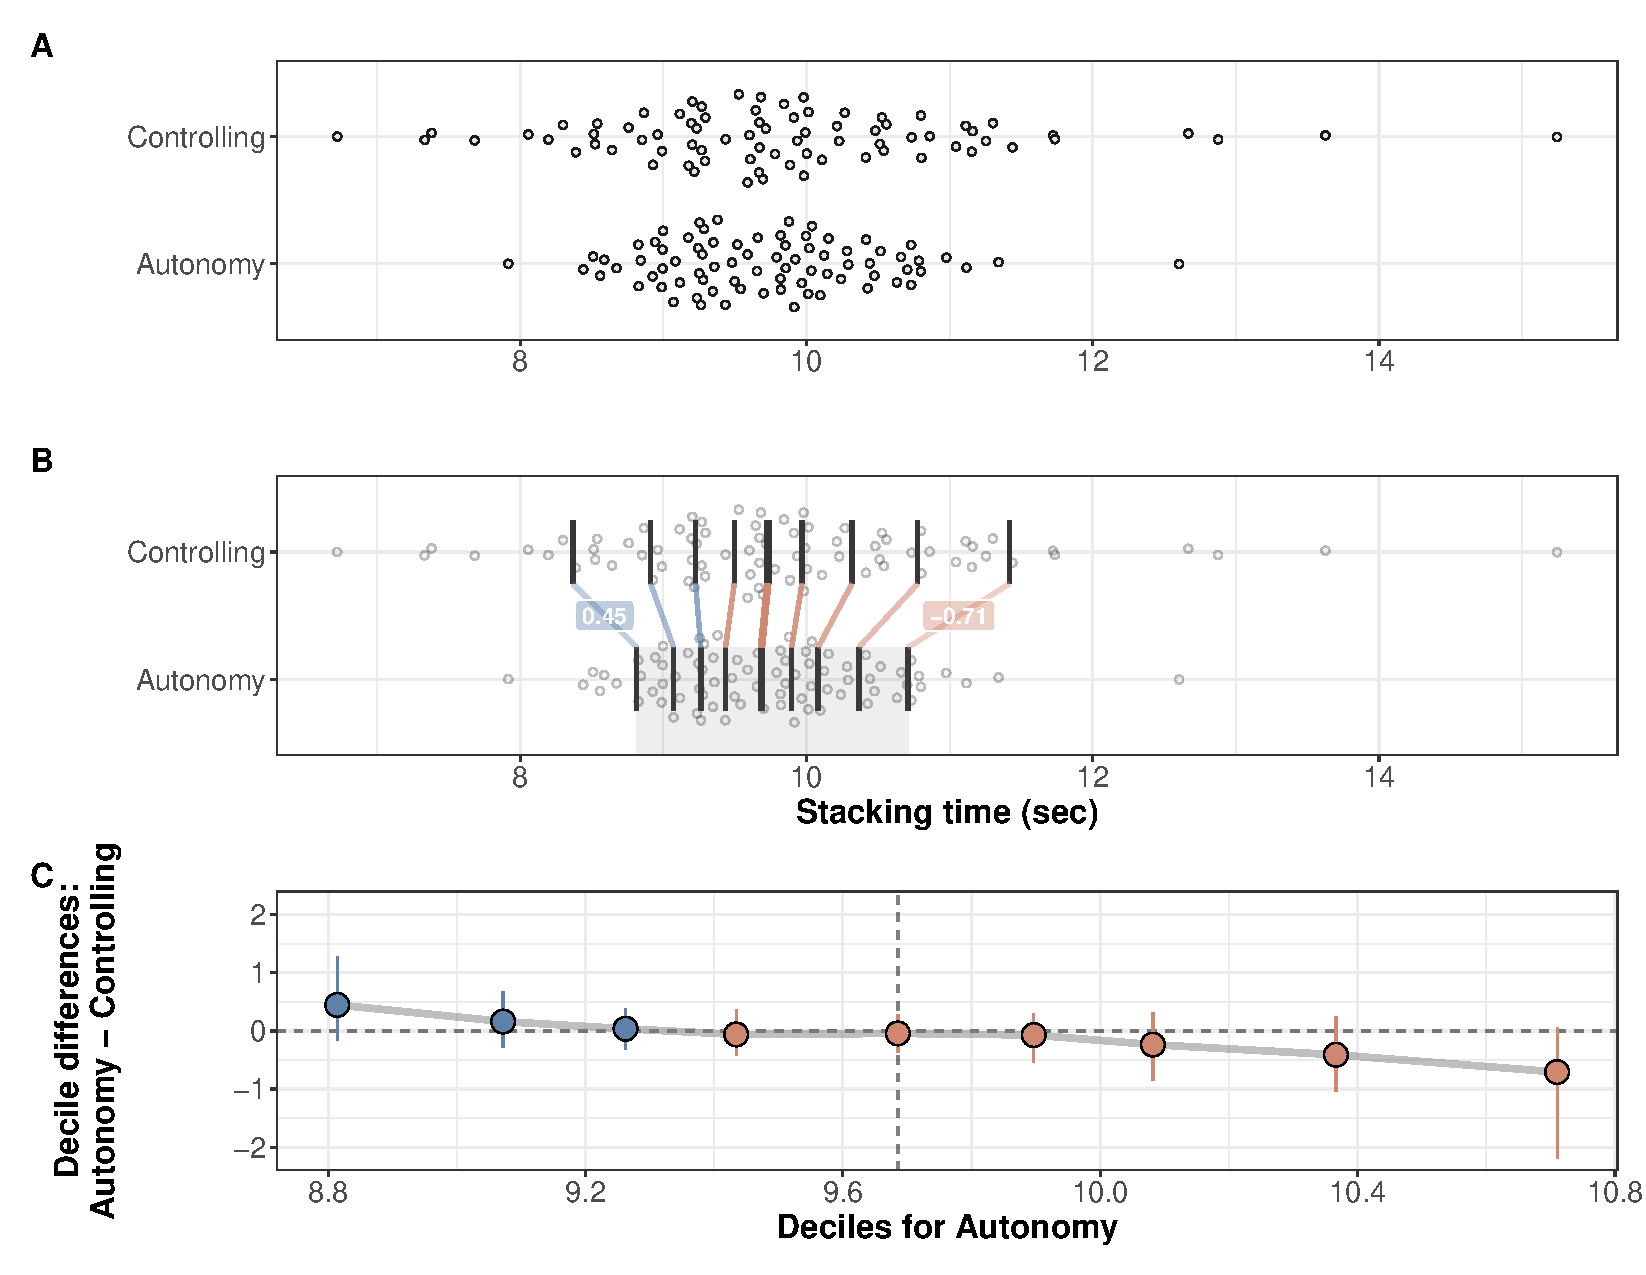
\includegraphics[scale=0.55]{../../figs/fig1.pdf}
    \setlength{\belowcaptionskip}{-2em}
    \caption*{\singlespacing \small Note. \normalfont Scatterplot of stacking time as a function of experimental group \textbf{(A)} with each data point representing a 20\% trimmed mean for an individual participant. The same scatterplot from the top row with the deciles if each distribution represented by the black lines \textbf{(B)}. The thick black line represents the median of each distribution. The difference between groups at each decile are represented by the colored lines. A blue line indicates that the Controlling language group was faster in a decile and an orange line indicates that the Autonomy-supportive language group was faster in a decile. The bottom row illustrates the shift function \textbf{(C)}, which focuses on the grey shaded region of the x-axis in the middle row. The deciles for the Autonomy-supportive language group are plotted on the x-axis and the difference in deciles between the two groups are plotted on the y-axis. The vertical dashed line represents the median of the Autonomy-supportive language group. The circles represent the decile differences using the same color coding described above. Error bars represent 95\% percentile bootstrapped confidence intervals. All decile comparisons were not significant after \emph{p}-values were adjusted for multiple comparisons using Hochberg's method.}
    \label{fig:fig1}
\end{figure}

\clearpage

\subsection{Secondary analyses}

\subsubsection{Acquisition phase}

We analyzed mean stacking time during the acquisition period using a 2 Group (Autonomy-support, Controlling) x 6 Block mixed design ANOVA with repeated measures on Block. Participants in the autonomy-supportive language and controlling language groups decreased their stacking time across acquisition blocks (Figure \ref{fig:fig2}). This was supported by a significant main effect of Block, $F(4.40, 677.96) = 111.91$, $p < .001$, $\eta_{G}^2 = .137$. Stacking time in Block 1 was slower than all other blocks ($p$'s < .001), Block 2 was slower than Blocks 3 to 6 ($p$'s $\leq$ .004), and Blocks 3 and 4 were both slower than Blocks 5 and 6 ($p$'s < .001). The main effect of Group, $F(1, 154) = 2.20$, $p = .140$, $\eta_{G}^2 = .011$, and the Group x Block interaction, $F(4.40, 677.96) = 0.59$, $p = .681$, $\eta_{G}^2 < .001$, were not significant.

\subsubsection{Retention test}

Performance in the delayed retention test was also analyzed using a more familiar approach in motor learning research. A one-tailed Welch's \emph{t}-test on pre-test adjusted mean stacking times for the Autonomy-supportive language group ($M = 9.86$ s, $SD = 0.80$) and the Controlling language group ($M = 10.04$ s, $SD = 1.37$) was not significant, $t(124.51) = 1.00$, $p = .159$, $d = .16$ $[-.156, .477]$. This finding is consistent with those of our primary analysis using the shift function.

\clearpage

\begin{figure}[htbp]
    \caption{Motor performance data for all experimental phases.}
    \centering
    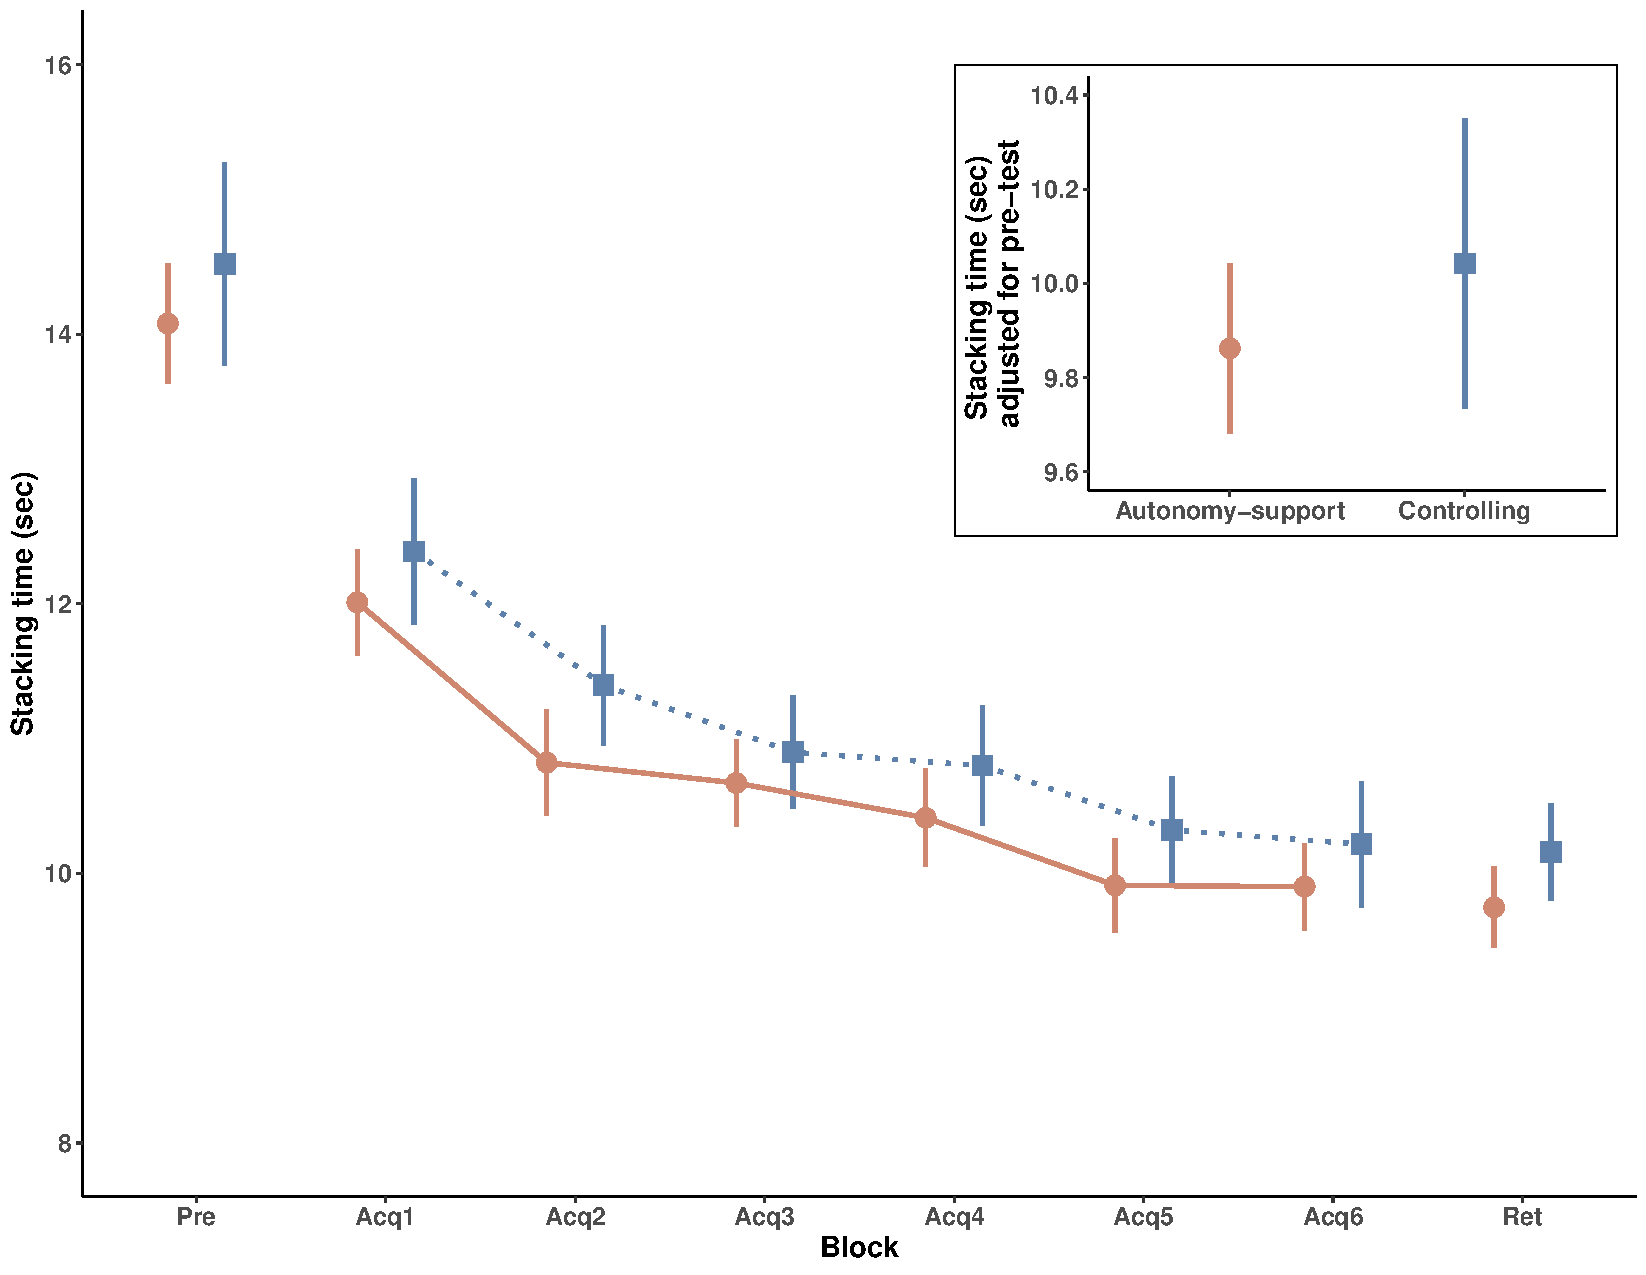
\includegraphics[scale=0.55]{../../figs/fig2.pdf}
    \setlength{\belowcaptionskip}{-2em}
    \caption*{\singlespacing \small Note. \normalfont Mean stacking time (s) for the Autonomy-supportive language (orange circles, solid line) and Controlling language (blue squares, dotted line) groups were computed by averaging the data into blocks of five trials. This resulted in one block for pre-test (Pre), six block for acquisition (Acq), and one block for the ~24-hr delayed retention test (Ret). The pre-test and acquisition blocks were completed in Session 1 and the retention block was completed in Session 2. Feedback about stacking time (s) was only available during the acquisition blocks and was provided after each trial. Group-specific instructions as a function of experimental group were played as pre-recorded audio clips before trials 1 (start of Block 1), 11 (start of Block 3), and 21 (start of Block 5) in acquisition. The inset figure shows pre-test adjusted retention stacking time (s) for both groups. Error bars in both figures represent 95\% confidence intervals.}
    \label{fig:fig2}
\end{figure}

\clearpage

\subsubsection{Psychological variables}

We assessed the impact of our instructional language manipulation on perceived autonomy, perceived competence, and intrinsic motivation using separate 2 Group (Autonomy-support, Controlling) x 2 Time (After acquisition, Before retention) mixed ANCOVAs with pre-test scores as the covariate and repeated measures on Time. 

Perceptions of autonomy (adjusted for pre-test) remained consistent within both groups (Figure \ref{fig:fig3}A). Pre-test, the covariate, was a significant predictor of later time points, $F(1, 153) = 247.68$, $p < .001$. Participants in the autonomy-supportive language group self-reported higher scores than the participants in the controlling language group after acquisition and before retention. This was supported by a significant main effect of Group, $F(1, 153) = 3.90$, $p = .05$, $\eta_{G}^2 = .022$. The main effect of Time, $F(1, 153) = 0.01$, $p = .924$, $\eta_{G}^2 < .001$, and the Group x Time interaction, $F(1, 153) = 1.13$, $p = .290$, $\eta_{G}^2 < .001$, were not significant.

Perceptions of competence (adjusted for pre-test) were relatively consistent in both groups (Figure \ref{fig:fig3}B). Pre-test was a significant predictor of later time points, $F(1, 153) = 231.31$, $p < .001$. Groups did not differ in their self-reported perceptions of competence. The main effects for Group, $F(1, 153) = 0.01$, $p = .933$, $\eta_{G}^2 < .001$, and Time, $F(1, 153) = 0.56$, $p = .456$, $\eta_{G}^2 < .001$, as well as the Group x Time interaction, $F(1, 153) = 0.38$, $p = .539$, $\eta_{G}^2 < .001$, were not significant.

Intrinsic motivation (adjusted for pre-test) scores remained consistent within both groups (Figure \ref{fig:fig3}C). Pre-test was a significant predictor of later time points, $F(1, 153) = 387.06$, $p < .001$. Groups did not differ in their self-reported intrinsic motivation. The main effects for Group, $F(1, 153) = 0.11$, $p = .743$, $\eta_{G}^2 < .001$, and Time, $F(1, 153) = 0.21$, $p = .605$, $\eta_{G}^2 < .001$, as well as the Group x Time interaction, $F(1, 153) = 0.13$, $p = .177$, $\eta_{G}^2 = .002$, were not significant.

\clearpage

\begin{figure}[htbp]
    \caption{Questionnaire data.}
    \centering
    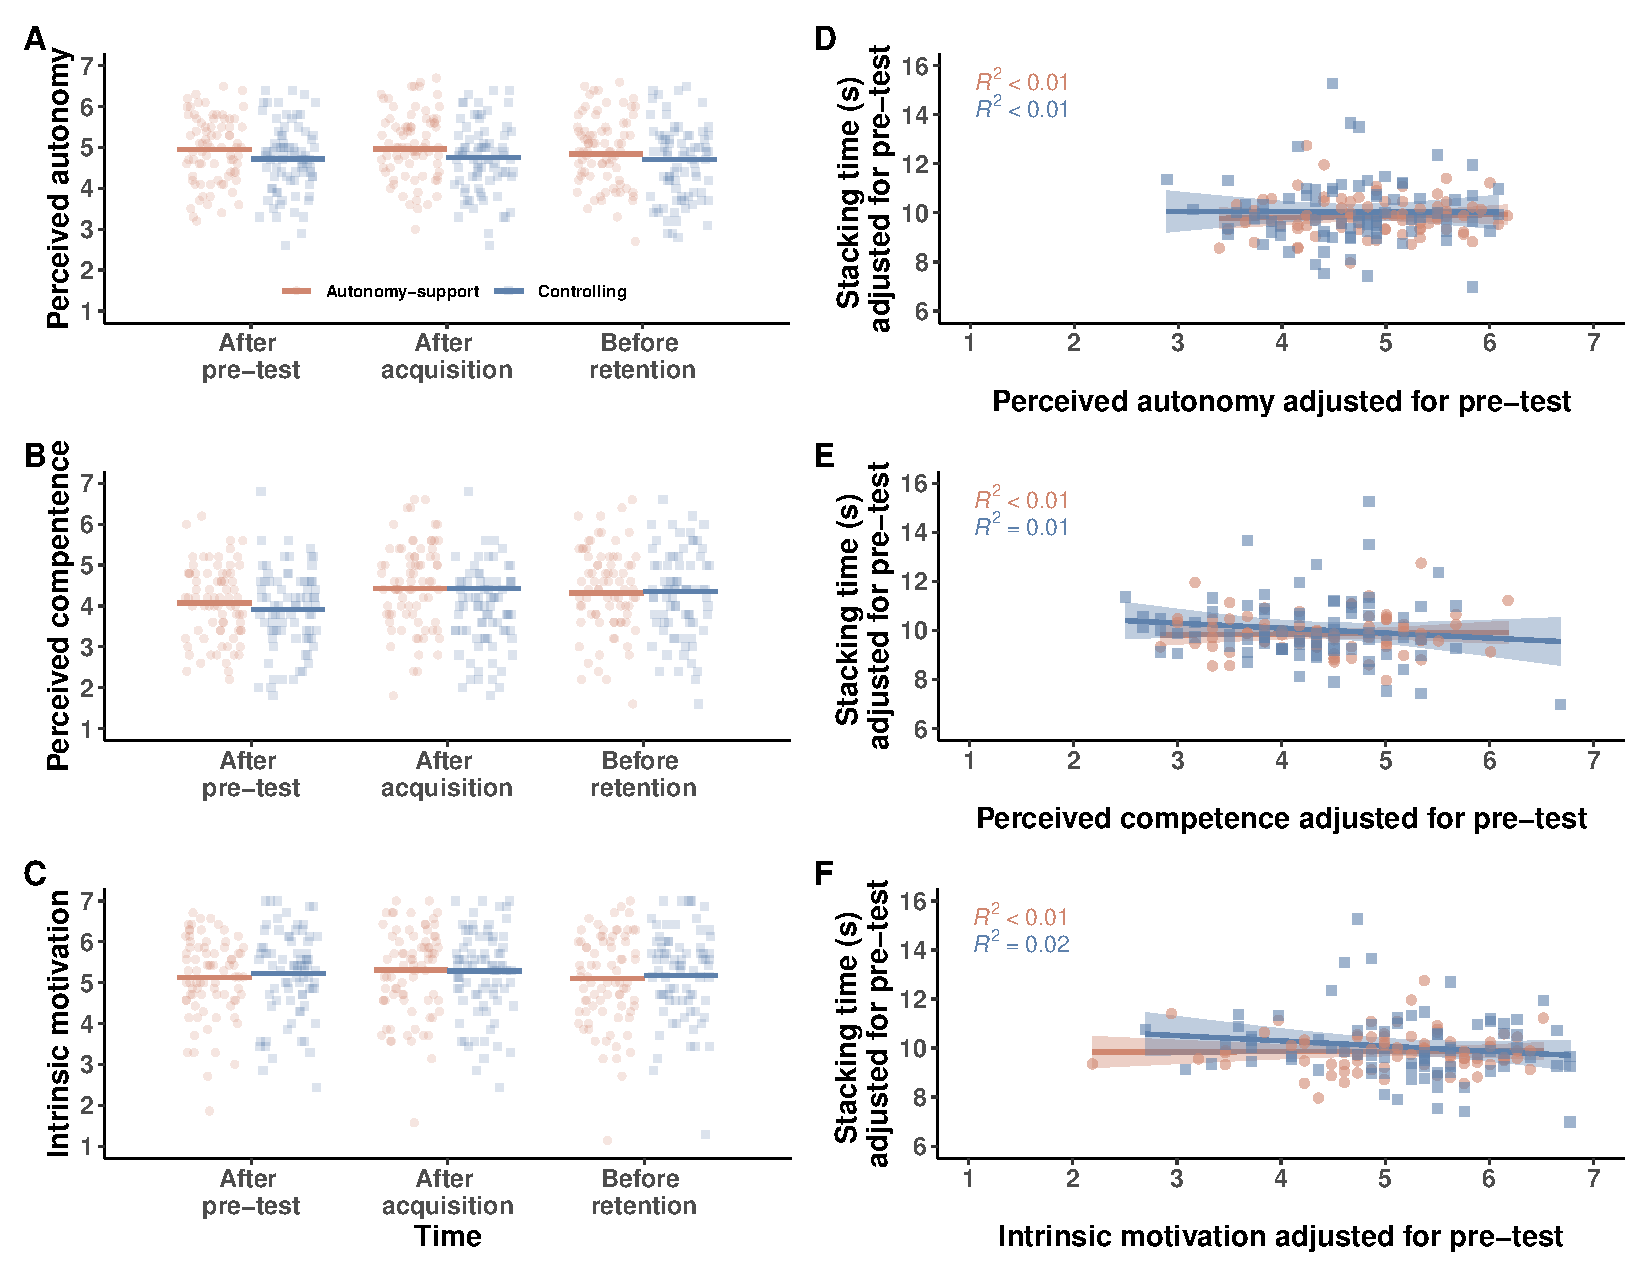
\includegraphics[scale=0.55]{../../figs/fig3.pdf}
    \setlength{\belowcaptionskip}{-2em}
    \caption*{\singlespacing \small Note. \normalfont Self-reported scores for perceived autonomy \textbf{(A)}, perceived competence \textbf{(B)}, and intrinsic motivation \textbf{(C)} after the pre-test, after the acquisition phase, and before the delayed retention test for the Autonomy-supportive language (orange circles) and the Controlling language (blue squares) groups. The horizontal bars represent the group means, with the pre-test adjusted mean shown for after acquisition and before retention. Each data point represents the mean score across subscale items for an individual participant. The relationship between retention stacking time (s) adjusted for pre-test and perceived autonomy \textbf{(D)}, perceived competence \textbf{(E)}, and intrinsic motivation \textbf{(F)} before retention and adjusted for pre-test is shown. Each data point represents the mean score across subscale items for an individual participant in the Autonomy-supportive language (orange circles) and the Controlling language (blue squares) groups. The estimated regression fit (solid lines) for each group is shown. The shaded areas represent the 95\% confidence intervals. A negative slope in these plots would suggest faster stacking times were associated with higher self-reported scores on the psychological variable of interest.}
    \label{fig:fig3}
\end{figure}

\clearpage

We also performed some exploratory correlational analyses between our three psychological variables and performance in retention. We plotted pre-test adjusted retention stacking times as a function of perceived autonomy (Figure \ref{fig:fig3}D), perceived competence (Figure \ref{fig:fig3}E), and intrinsic motivation (Figure \ref{fig:fig3}F) scores before retention, adjusted for pre-test for each participant. If there were associations between these psychological variables and performance in retention, we expected to see a negative relationship (i.e., faster stacking times associated with higher self-reported scores). As can be seen, we instead found the relationships between retention performance and each psychological variable to be relatively flat.

\subsection{Equivalence test}

Due to the null findings of the shift function (and \emph{t}-test) on retention stacking times, we tested for equivalence with a noninferiority test as outlined in our preregistration. We used the two one-sided test procedure \autocite{schuirmann1987} and a noninferiority bound of $d = .4$, which was our smallest effect size of interest. The test was not significant, $t(124.5) = 1.50$, $p = .069$. The 90\% confidence interval around the effect size in retention was [-.11, .43], indicating that these data are inconsistent with all effects larger than $d = \pm.43$.

\section{Discussion}

In their OPTIMAL theory of motor learning, \textcite{wulf2016} suggested that motor performance and learning can be enhanced when learners receive task instructions that use autonomy-supportive rather than controlling language. Here, we investigated the effect of autonomy-supportive instructional language on the acquisition and retention of a speed cup stacking task. Based on the OPTIMAL theory, we predicted that participants in the autonomy-supportive language group would demonstrate faster stacking times in acquisition and delayed retention, and would also report higher perceptions of autonomy, competence, and intrinsic motivation compared to those in the controlling language group. Our results did not show a performance benefit from autonomy-supportive language in acquisition or retention compared to controlling language. We found significantly higher perceptions of autonomy in the autonomy-supportive language group compared to the controlling language group, but no significant group differences for perceived competence or intrinsic motivation. Taken together, our findings do not support key predictions of the OPTIMAL theory of motor learning.

We failed to replicate the performance advantage of autonomy-supportive language in acquisition and delayed retention compared to controlling language that was reported by \textcite{hooyman2014}. This is also inconsistent with Wulf and Lewthwaite's (\citeyear{wulf2016}) OPTIMAL theory wherein task instructions that utilize autonomy-supportive language results in a virtuous cycle that has positive influences on motor performance and learning. Importantly, our failed replication and lack of support for OPTIMAL theory are not the result of participants failing to improve at the motor task or an unsuccessful instructional language manipulation. That is, both the autonomy-supportive language and controlling language groups showed a decrease in stacking times from pre-test to the delayed retention test, suggesting learning occurred (see Figure \ref{fig:fig2}) and the autonomy-supportive language group reported higher perceptions of autonomy (see Figure \ref{fig:fig3}A). These conflicting findings may be due to the previously identified methodological limitation in \textcite{hooyman2014} of a small sample size or potential flexibility in the data analysis as their experiment was not pre-registered. Although such factors may have contributed, we believe the main reason for our discrepant results arise from the confounding analogy included in Hooyman and colleagues' (\citeyear{hooyman2014}) autonomy-supportive instructions, but excluded from both their controlling and neutral language instructions. It is therefore possible that their "autonomy-supportive language advantage" was \emph{actually} an analogy advantage \autocite[e.g.,][]{liao2001,masters2020}. This possibility clearly highlights the importance of carefully crafting instructions that only differ in terms of the primary predictor variable of interest, instructional language, in future research.

Despite having the largest sample size in an instructional language motor learning experiment to date, the results of our robust shift function, a more traditional \emph{t}-test, and non-inferiority test were inconclusive. Using our smallest effect size of interest ($d = .4$) as the noninferiority bound, the effect size at delayed retention in the present experiment is inconsistent with all effects larger than $d = \pm.43$. Although this is bigger than our pre-registered smallest effect size of interest, this test would reject the median effect size previously found in motor learning research \autocite[\emph{d} = .63 by][]{lohse2016}. As such, future research investigating the impact of instructional language on motor skill acquisition likely requires larger sample sizes than that used in the present experiment and what is commonly found in motor learning research \autocite[see][for discussions]{lohse2016,mckay2023}. As such, it is critical that motor learning scientists justify their sample sizes in future research \autocite[e.g.,][]{lakens2022,mckay2023a} and when using \emph{a priori} power analyses to ensure all relevant information is reported in a reproducible manner \autocite{mckay2023b}.

When examining the stacking time distributions for each group in retention (see Figure \ref{fig:fig1}A), it is clear that the spread of the data in the two distributions is different. Such differences can be masked when researchers only use standard summary statistics such as the mean \autocite[see][for the famous Anscombe's quartet example]{anscombe1973}. Although all adjusted decile comparisons in our primary shift function analysis were not significant, there were some interesting trends that could have theoretical and/or practical significance for future work. Specifically, there was a trend for better performance with controlling language for the participants who were in the fastest (i.e., more skilled) stacking time decile (unadjusted $p = .051$) and a trend for better performance with autonomy-supportive language for the participants who were in the slowest (i.e., less skilled) stacking time decile (unadjusted $p = .017$). This pattern suggests that the motor learning benefits of different instructional language wording may potentially interact with skill level; however, a large \emph{N} experiment would be required to adequately test this hypothesis. If this hypothesis could be empirically supported, it would be incompatible with OPTIMAL theory as \textcite{wulf2016} predicted that autonomy-supportive instructional language is beneficial irrespective of skill level. A possible explanation for why less skilled individuals could benefit from autonomy-supportive instructions compared to more skilled individuals benefiting from controlling language instructions is that the former may act as a buffer against poor performance by allowing learners to persevere and remain engaged in the task during practice. Thus, future work in this area should consider including behavioural, neural, and/or psychological measures related to task engagement \autocite[e.g.,][]{fairclough2009,leiker2016,obrien2009}. Additionally, motor learning scientists may want to consider leveraging modern and robust statistical tools \autocite{wilcox2021} in their work as these techniques may provide greater insight and a more nuanced understanding of their data.

Despite the prominent role of autonomy-support facilitating motor performance and learning in OPTIMAL theory, the higher perceptions of autonomy in our autonomy-supportive language group (see Figure \ref{fig:fig3}A) did not translate into superior performance in either acquisition or retention compared to the controlling language group. The higher reported perceived autonomy scores in the autonomy-supportive language group serves as a manipulation check and is also consistent with findings from previous research \autocite[e.g.,][]{reeve2011} and multiple meta-analyses \autocite[e.g.,][]{mossman2022,ng2012,okada2021,su2011}. However, our estimate of this effect on perceptions of autonomy is much smaller than previous estimates. The estimated size in the present experiment is $d = .27$ [.05, .49], which is outside the 95\% confidence interval around Su and Reeve's (\citeyear{su2011}) estimate of $d = .63$ [.43, .83]. A potential explanation for our smaller estimate is that \textcite{su2011} identified five components that can make instructions autonomy-supportive: 1) use non-controlling language, 2) acknowledge negative feelings, 3) nurture inner motivational resources, 4) provide meaningful rationales, and 5) offer choices; and many of the experiments in their meta-analysis included either four or all five components. In contrast, our instructions only included the first three components. Although this suggests that not all components may be necessary to have a positive influence on perceptions of autonomy, the strength of the effect may scale with the number of components incorporated in the instructions. This may be important for seeing differences in motor performance and learning. Future research would be needed to test this possibility. Another possibility for the smaller effect size and lack of performance differences in acquisition and retention is that participants received the same pre-recorded, group-specific instructions throughout practice. During skill acquisition outside of a lab, coaches likely alter the wording of their instructions in a more dynamic way to meet an athlete's needs. Thus, future research could test this idea by having slight variations in the instructions each time they are provided to the learners during acquisition.

In OPTIMAL theory, autonomy-support is also predicted to facilitate performance by enhancing expectancies. We did not find support for this prediction in the present experiment as there were no group differences in self-reported perceptions of competence (see Fig. \ref{fig:fig3}B). This differs from \textcite{hooyman2014} who reported enhanced expectancies following autonomy-supportive instructional language compared to their controlling language group. A potential explanation for this discrepancy in findings might relate to measuring different psychological constructs as proxies for enhanced expectancies. Specifically, we measured perceptions of competence whereas Hooyman and colleagues measured self-efficacy. It is worth noting that the positive effect on self-efficacy in \textcite{hooyman2014} was quite transient as this difference between autonomy-supportive and controlling language on Day 1 did not persist on Day 2 in their experiment.\footnotemark Another potential reason for our differences with Hooyman and colleagues might relate to task performance during practice. \textcite{hooyman2014} found superior performance in the autonomy-support group compared to the controlling language group during acquisition, which likely contributed to them reporting higher self-efficacy. In contrast, we did not find a group difference in task performance during practice. When considering this, it is perhaps not too surprising that we did not find differences in perceptions of competence when actual task performance was similar between our autonomy-supportive and controlling language groups. We also did not find higher instrinsic motivation in the autonomy-supportive language group compared to the controlling language group (see Fig. \ref{fig:fig3}C), a finding that is consistent with recent large \emph{N}, and often preregistered, experiments investigating the role of autonomy-supportive manipulations on motor learning \autocite[e.g.,][]{bacelar2022,stgermain2022,stgermain2023}. Lastly, we did not see the expected relationship between self-reported scores for any of the measured psychological constructsbefore retention with performance on the delayed retention test (see Figs. \ref{fig:fig3}D-F). Taken together, these findings are difficult to reconcile with key predictions in OPTIMAL theory \autocite{wulf2016} where autonomy-supportive practice conditions should enhance expectancies and increase intrinsic motivation relative to autonomy-thwarting practice conditions.

A potential limitation of the current experiment is the lack of a neutral language group. We did not include a neutral language group for several reasons. First, the inclusion of a third group would have substantially increased the required sample size (from \emph{N} = 156 to \emph{N} = 246) to investigate our smallest effect size of interest with adequate power. Second, as such an increase in sample size would have exceeded our resource constraints \autocite{lakens2022,lenth2001}, we instead decided to conduct a large \emph{N} experiment that focused on the ends of the instructional language continuum, or in other words, the biggest potential difference. Third, in both \textcite{reeve2011} and \textcite{hooyman2014}, the key differences were between the autonomy-supportive language group and the controlling language group. Lastly, autonomy-supportive and controlling language are often used in real-world settings such as physiotherapy \autocite[e.g.,][]{murray2015} and  coaching \autocite[e.g.,][]{bartholomew2009,carroll2021}, with little inclusion of neutral language. For these reasons, we contend that a neutral language group would not have added enough value to offset the costs associated with the substantial increase in sample size. Another potential limitation is that although our autonomy-supportive manipulation was significant, the estimated magnitude of this effect was quite small relative to past research. We attribute this difference to our much larger sample size compared to other motor learning research \autocite[e.g.,][]{hooyman2014}, which allowed for greater precision in our estimates. Nevertheless, future research in this area should continue to use large \emph{N} designs paired with all five components that can make instructions autonomy-supportive as identified by \textcite{su2011}.

In conclusion, we did not find a motor performance and learning advantage of instructions with autonomy-supportive language compared to controlling language. This finding is inconsistent with past motor learning research \autocite[e.g.,][]{hooyman2014} and the OPTIMAL theory of motor learning \autocite{wulf2016}. Despite no motor performance or learning differences, we did find higher perceptions of autonomy in the participants that received autonomy-supportive instructional language compared to those that received controlling instructional language. While the primary goal of most motor learning interventions is a relatively permanent change in the capability for skill \autocite{schmidt2019}, it is worth noting that in some situations autonomy-support in and of itself might be a desired affective outcome \autocite[e.g.,][]{stemarie2020a}. In such situations, autonomy-supportive instructional language could be paired with another form of practice that has more reliable effects on motor learning. Our perceived competence and intrinsic motivation data were also not consistent with OPTIMAL theory. While we do not discount the importance of motivation for motor skill acquisition, based on the current data we suggest that these motivational factors may instead have an \emph{indirect} \autocite[e.g.,][]{salmoni1984} rather than the argued \emph{direct} \autocite[e.g.,][]{wulf2016} influence on motor skill learning.

\clearpage

\subsection{Author contributions (CRediT Taxonomy)}

\noindent Conceptualization: LSG, BM, DMYB, MJC \newline
\noindent Data curation: LSG, MJC \newline
\noindent Formal analysis: LSG \newline
\noindent Funding acquisition: LSG, MJC \newline
\noindent Investigation: LSG, LB, CT, JS, CC \newline
\noindent Methodology: LSG, BM, MJC \newline
\noindent Project administration: LSG, MJC \newline
\noindent Software: LSG, BM, MJC \newline
\noindent Supervision: MJC \newline
\noindent Validation: BM, DMYB, MJC \newline
\noindent Visualization: LSG, MJC \newline
\noindent Writing -- original draft: LSG, BM, LB, CT, JS, CC, DMYB, MJC \newline
\noindent Writing -- review \& editing: LSG, BM, LB, CT, JS, CC, DMYB, MJC

\subsection{Declaration of competing interest}

\noindent All authors have no competing interests to declare.

\subsection{Availability of data and code}

\noindent Data and scripts are available at \url{https://github.com/cartermaclab/expt_instructional-language}.

\subsection{Funding}

\noindent This work was supported by the Natural Sciences and Engineering Research Council (NSERC) of Canada (RGPIN-2018-05589; MJC) and McMaster University (MJC). LSG was supported by an NSERC Postgraduate Scholarship.

\clearpage

\printbibliography

\end{document}